\documentclass[tikz, border=10pt]{standalone}
\usepackage{tikz}
\usetikzlibrary{positioning, arrows.meta, decorations.pathreplacing}

\definecolor{inputcolor}{RGB}{70, 130, 180}
\definecolor{hiddencolor}{RGB}{60, 179, 113}
\definecolor{outputcolor}{RGB}{220, 80, 80}
\definecolor{labelcolor}{RGB}{80, 80, 80}

\begin{document}
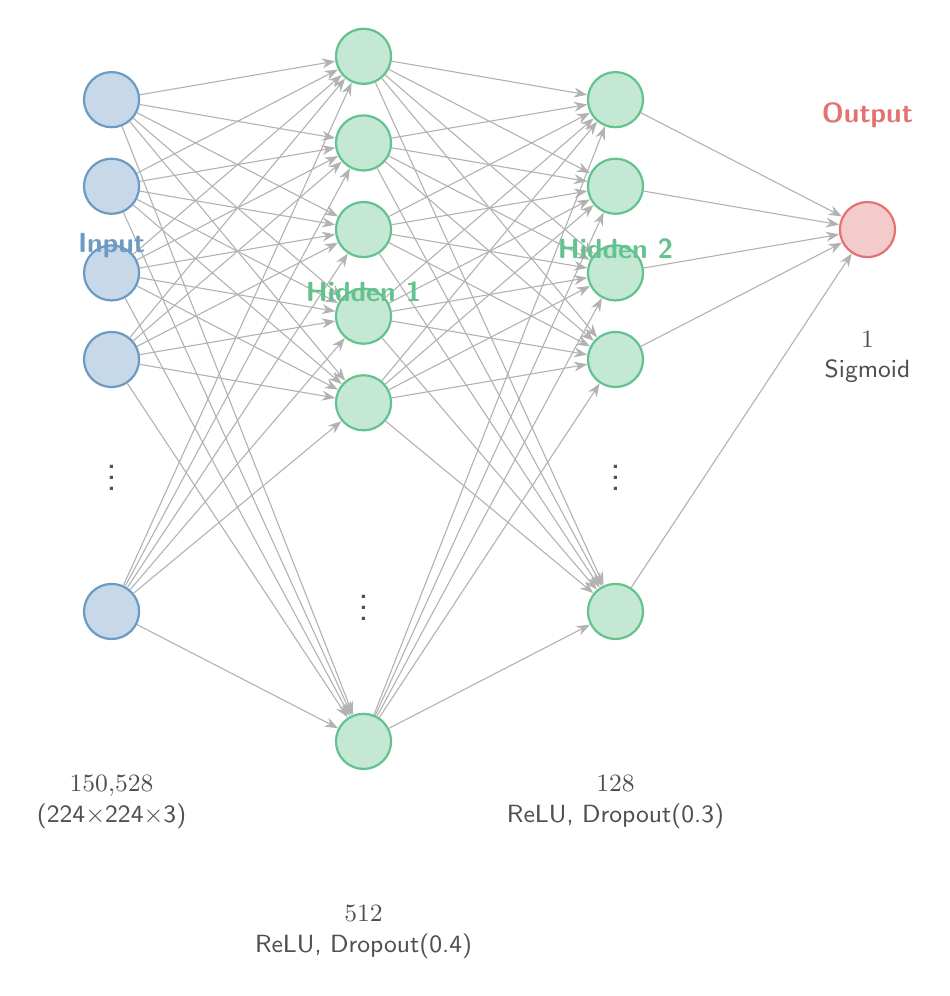
\begin{tikzpicture}[
    neuron/.style={circle, draw, minimum size=0.7cm, line width=0.8pt, font=\small},
    input neuron/.style={neuron, fill=inputcolor!30, draw=inputcolor!80},
    hidden neuron/.style={neuron, fill=hiddencolor!30, draw=hiddencolor!80},
    output neuron/.style={neuron, fill=outputcolor!30, draw=outputcolor!80},
    annot/.style={font=\small\sffamily, text=labelcolor},
    arrow/.style={->, >=Stealth, gray!60, line width=0.4pt},
]

% --- Layer x-positions ---
\def\layerI{0}
\def\layerII{3.2}
\def\layerIII{6.4}
\def\layerIV{9.6}

% --- Number of visible neurons per layer ---
\def\nI{5}   % input  (+ dots)
\def\nII{6}  % hidden1
\def\nIII{5} % hidden2
\def\nIV{1}  % output

% ======= INPUT LAYER =======
\foreach \i in {1,...,4} {
    \node[input neuron] (I-\i) at (\layerI, {(\i-2.5)*1.1}) {};
}
\node[annot] (I-dots) at (\layerI, {(0-2.5)*1.1 - 0.3}) {\Large$\vdots$};
\node[input neuron] (I-5) at (\layerI, {(-1-2.5)*1.1 - 1.0}) {};

% ======= HIDDEN LAYER 1 =======
\foreach \i in {1,...,5} {
    \node[hidden neuron] (H1-\i) at (\layerII, {(\i-3)*1.1}) {};
}
\node[annot] (H1-dots) at (\layerII, {(-1-3)*1.1 - 0.3}) {\Large$\vdots$};
\node[hidden neuron] (H1-6) at (\layerII, {(-2-3)*1.1 - 1.0}) {};

% ======= HIDDEN LAYER 2 =======
\foreach \i in {1,...,4} {
    \node[hidden neuron] (H2-\i) at (\layerIII, {(\i-2.5)*1.1}) {};
}
\node[annot] (H2-dots) at (\layerIII, {(0-2.5)*1.1 - 0.3}) {\Large$\vdots$};
\node[hidden neuron] (H2-5) at (\layerIII, {(-1-2.5)*1.1 - 1.0}) {};

% ======= OUTPUT LAYER =======
\node[output neuron] (O-1) at (\layerIV, 0) {};

% ======= CONNECTIONS =======
% Input -> H1
\foreach \i in {1,...,4} {
    \foreach \j in {1,...,5} {
        \draw[arrow] (I-\i) -- (H1-\j);
    }
    \draw[arrow] (I-\i) -- (H1-6);
}
\foreach \j in {1,...,5} {
    \draw[arrow] (I-5) -- (H1-\j);
}
\draw[arrow] (I-5) -- (H1-6);

% H1 -> H2
\foreach \i in {1,...,5} {
    \foreach \j in {1,...,4} {
        \draw[arrow] (H1-\i) -- (H2-\j);
    }
    \draw[arrow] (H1-\i) -- (H2-5);
}
\foreach \j in {1,...,4} {
    \draw[arrow] (H1-6) -- (H2-\j);
}
\draw[arrow] (H1-6) -- (H2-5);

% H2 -> Output
\foreach \i in {1,...,4} {
    \draw[arrow] (H2-\i) -- (O-1);
}
\draw[arrow] (H2-5) -- (O-1);

% ======= LAYER LABELS (top) =======
\node[annot, above=0.8cm of I-1,  font=\bfseries\sffamily, text=inputcolor!80]  {Input};
\node[annot, above=0.8cm of H1-1, font=\bfseries\sffamily, text=hiddencolor!80] {Hidden 1};
\node[annot, above=0.8cm of H2-1, font=\bfseries\sffamily, text=hiddencolor!80] {Hidden 2};
\node[annot, above=0.8cm of O-1,  font=\bfseries\sffamily, text=outputcolor!80] {Output};

% ======= SIZE ANNOTATIONS (below) =======
\node[annot, below=1.6cm of I-5,  align=center] {$150{,}528$\\(224$\times$224$\times$3)};
\node[annot, below=1.6cm of H1-6, align=center] {$512$\\ReLU, Dropout(0.4)};
\node[annot, below=1.6cm of H2-5, align=center] {$128$\\ReLU, Dropout(0.3)};
\node[annot, below=0.8cm of O-1,  align=center] {$1$\\Sigmoid};

\end{tikzpicture}
\end{document}
